\section{Señales}
\subsection{Fundamentos de las señales}
Las señales que se envían por el canal físico para comunicar dos extremos de un canal son \textbf{ondas electromagnéticas} que se propagan a través del canal a una cierta velocidad determinada por el tipo de canal que estemos usando.


Podemos definir todas las señales con una función períodica \(f(t)\) llamada \textbf{frecuencia}. Esto significa que \(f(t) = f(t + T)\) para alguna constante \(T\). Al minimo valor positivo mayor que cero de \(T\) que cumple esto, lo llamamos \textbf{período fundamental}. \(f\) se mide en Hertz o ciclos por segundo y \(T\) en segundos. 

En base a a la frecuncia y el período de una onda definimos:

\begin{itemize}
  \item \textbf{Amplitud:} Indica la cantidad de cambios en la presión del aire. Se mide en decibeles (db o volts). Por decirlo de otra forma, la amplitud es la distancia entre el eje horizontal y el punto más alto del pico de la onda, o el punto más bajo de la depresión de la onda.
  \item \textbf{Frecuencia angular:} \(\omega = 2\pi f\) radianes por segundos.
  \item \textbf{Fase \(\phi\)}: Compara el tiempo entre dos ondas y se mide en grados, de 0 a 360. Cuando dos ondas comienzan al mismo tiempo, se dice que están en fase o alineadas en fase. Cuando una onda se encuentra ligeramente retrasada en comparación con otra onda, se dice que las ondas están desfasadas.
  \item \textbf{Longitud de onda:} Es la distancia entre los ciclos repetitivos de una onda a una frecuencia dada. Cuanto más elevada sea la frecuencia, más corta será la longitud de onda: \[\lambda = \frac{c}{f}\]
  donde \(c=3*10^8\frac{m}{s}\) es la velocidad de la luz.
\end{itemize}
\begin{figure}[H]
	\centering
	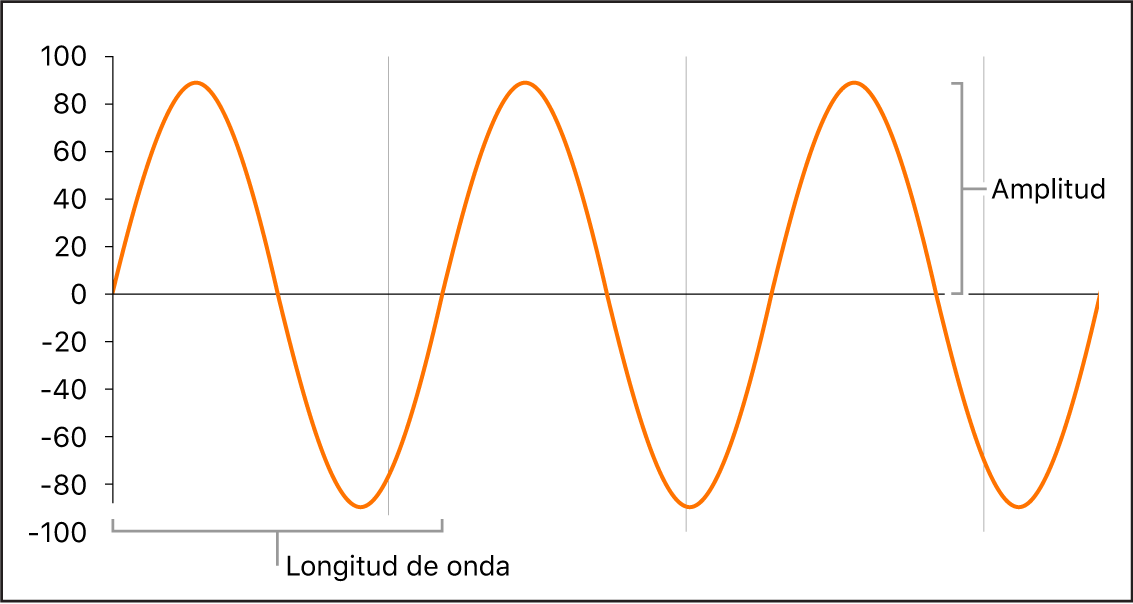
\includegraphics[width=0.65\textwidth
]{images/amplitud.png}
	\caption[Onda de señal]{Onda de señal}
	\label{fig:sistema-comunicacion-real}
\end{figure}

Esta onda puede chocar con imperfecciones del material (del canal), producir reflexiones y refracciones que se traducen en \textbf{perdidas} (menos energía para la señal original en la que está codificado el mensaje)

Dado que las ondas electromagnéticas son continuas y que son modificadas a medida que se propagan por el canal, debemos encontrar una manera de mapear estas frecuencias a los 0 y 1 que componen nuestros mensajes.

Para esto, tanto el transmisor como el recibidor definen un \textbf{ancho de banda} que es el rango de frecuencias que va a ocupar las señales que van a ser transmitidas por el canal y dentro de ese rango, cuales deben ser mapeadas a un 1 y cuales a un 0.

\subsection{Transformación de fourier}
Todas las funciones períodicas pueden expresarse como una suma infinita de senos y cosenos:

\[f(t) = \frac{1}{2}c + \sum_{i=0}^\infty \left(a_i\sen(n\omega t) + b_i\cos(n\omega t)\right)\]

done \(\omega\) es la frecuencia angular y \(a_i\) es la amplitdud de la onda.

Ninguna instalación transmisora puede transmitir señales sin perder cierta potencia en el proceso. Si todos los componentes de Fourier disminuyeran en la misma proporción, la señal resultante se reduciría en amplitud, pero no se distorsionaría. Desgraciadamente, todas las instalaciones de transmisión disminuyen los distintos componentes de Fourier en diferente grado, lo que provoca distorsión. Por lo general, las amplitudes se transmiten sin ninguna disminución desde 0 hasta cierta frecuencia \(f_c\) y todas las frecuencias que se encuentren por arriba de esta frecuencia de corte serán atenuadas. El rango de frecuencias que se transmiten sin atenuarse se conoce como \textbf{ancho de banda}. En la práctica, el corte no es abrupto, por lo que, en general, el ancho de banda ofrecido va desde 0 hasta la frecuencia en la que el valor de la amplitud es atenuado a la mitad de su valor original.

El ancho de banda es una propiedad física del medio de transmisión y por lo general depende
de la construcción, grosor y longitud de dicho medio. En algunos casos, se introduce un filtro en el
circuito para limitar la cantidad de ancho de banda disponible para cada cliente.

\subsection{Problemas de los medios de transmisión reales}
Cuando enviamos un mensaje a una máquina en una red, debemos pasar ese mensajes por un \textbf{transmisor} que convertirá el mensaje en una serie de \textbf{señales} que pueden ser enviadas a través del \textbf{canal} que nos comunica con la máquina de \textbf{destino}. La máquina de destino debe tener un \textbf{recibidor} que le permita captar las señales del canal y transformarlas nuevamente en el mensaje original.

Sin embargo, los canales de transmisión físicos no son perfectos y aportan \textbf{ruido} a las señales emitidas por nuestro transmisor pudiendo llegar a destino con errores.

\begin{figure}[H]
	\centering
	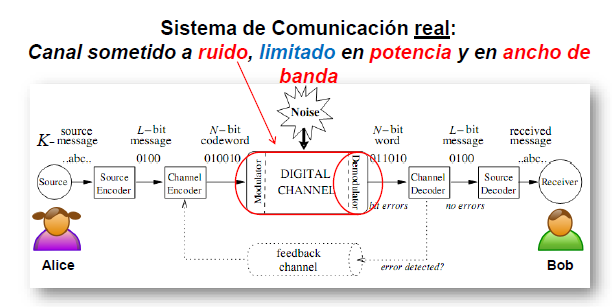
\includegraphics[width=0.65\textwidth
]{images/sistema-comunicacion-real.png}
	\caption[Esquema general de un sistema de comunicación]{Esquema general de un sistema de comunicación}
	\label{fig:sistema-comunicacion-correccion}
\end{figure}

Una forma de tratar de resolver esto es agregar al modelo nuevas capas de actores que trabajan para reducir los efectos nocivos del ruido. Por ejemplo, podemos agregar al modelo observadores externos que sean capaces de ver lo que se transmite de un lado y se recibe del otro, deducir información a partir de las diferencias, y tener chance de enviarle
correcciones al Elemento Corrector. También es posible tener dos niveles de observadores:
uno que se maneja a nivel mensaje y otro que se maneja a nivel característica del canal
propio.

\subsubsection{Tipos de errores de los canales físicos}
\begin{itemize}
  \item \textbf{Atenuación:}  En medios análogicos, la señales se degradan con la distancia recorrida lo que puede llevar a provocar errores en algunos bits recibidos. Por lo que la intensidad de la señal recibida deber ser suficiente para ser detectada y, además, debe ser suficientemente mayor al ruido del canal para que se reciba sin error. En general, las frecuencias más afectadas son las más altas por lo que se puede ecualizar estas frecuencias, es decir, amplificarlas.
  \item \textbf{Distorsión de retardo:} En medios guiados, la velocidad de propagación en el medio varía con la frecuencia por lo que los componentes del mensaje llegan en distintos instantes de tiempo, originando desplazamiento de fases entre las distintas frecuencias. Esto se puede deber a varios motivos.
\item \textbf{Ruido:} Los canales físicos poseen ruido natural. Es decir, transmiten señales adicionales debido a agentes externos:
\begin{itemize}
  \item \textbf{Ruido Término ó Ruido Blanco:} Se produce debido a la agitación térmica de electrones y aumenta linealmente con la temperatura absoluta del canal. En general, está distribuido de manera uniforme a lo largo de todo el canal y para un ancho de banda \(B\), la potencia del ruido blanco \(N_b = kTB\). 
  \item\textbf{Ruido por intermodulación:} Son señales que son la suma o la diferencia de sus frecuencias originales producidas por una falta de linealidad en el canal. \(N_I = m f_1 \pm n f_2\)
  \item\textbf{Ruido por Diafonía:} Se produce cuando una señal de una línea interfiere en otra.
  \item\textbf{Ruido impulsivo:} Son impulsos irregulares o picos que se pueden producir por interferencias externas (como pueden ser interferencia electromagnéticas, tormentas, etc). Este tipo de ruido es de corta duración, tienen gran amplitud y es disruptivo.
\end{itemize}
\end{itemize}

\subsubsection{Capacidad de un canal}
Las perturbaciones mencionadas afectan la velocidad de transmición del canal por lo que debemos asegurarnos de no enviar más bits que la capacidad límite del mismo para no perder información durante la transmición. Para esto vamos a definir los siguientes conceptos:

\begin{itemize}
  \item \(C\) es la capacidad del canal o tasa de datos, es decir a la cantidad de bits por segundo que podemos transmitir a través del mismo.
  \item \(B\) es el ancho de banda por el cual vamos a transmitir nuestros datos, va estar medido en ciclos por segundo (Hertz) y va estar limitado por el transmisor y el medio.
  \item \(N\) es el nivel medio o potencia del ruido del canal
  \item \(BER\) es la tasa de errores de bits por segundo (Bit Error Rate).
  \item \(S\) es la potencia o amplitud de la señal.
  \item \(SNR = S / N\) es la cantidad de ruido térmico presente se mide por la relación entre la potencia de la señal y la potencia del ruido, llamada relación señal a ruido. Por lo general, la relación misma no se expresa; en su lugar, se da la cantidad \(10 \log_{10} S/N\).
  Estas unidades se conocen como decibeles (dB).
\end{itemize}

En un canal sin ruido, \(C = 2B\log_2 M\) donde \(M\) es la cantidad de niveles que usamos para representar los símbolos.

En un canal con ruido, Shannon propuso
\[C_{max} = B\log_2(1 + SNR)\]

En principio, si se aumentan el ancho de banda \(B\) y la potencia de señal \(S\), aumenta la velocidad binaria. Sin embargo, un aumento de \(B\) aumenta el ruido y un aumento de \(S\) aumenta las no linealidades y el ruido de intermodulación.

\begin{figure}[H]
	\centering
	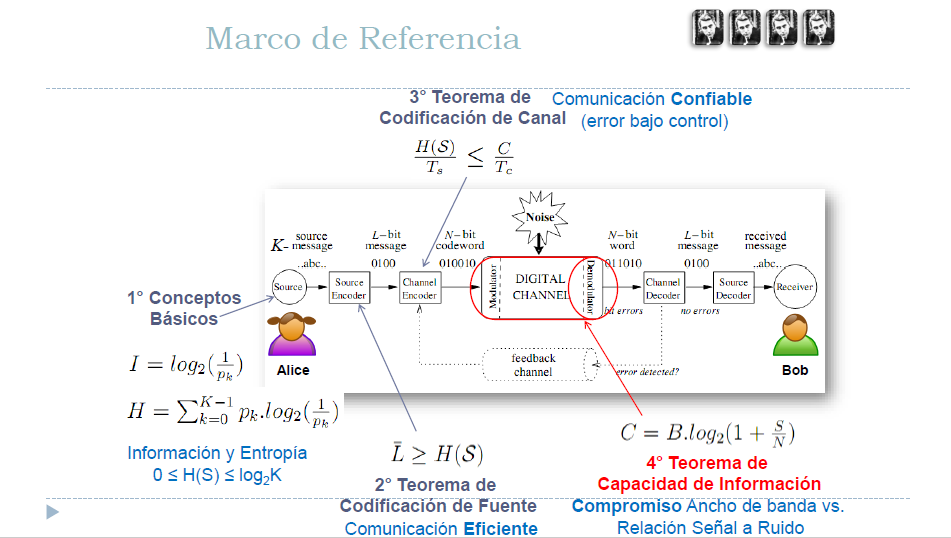
\includegraphics[width=\textwidth
]{images/marco-referencia.png}
	\caption[Esquema de un sistema de comunicación y sus conceptos asociados]{Esquema de un sistema de comunicación y sus conceptos asociados}
	\label{fig:marco-referencai}
\end{figure}


\paragraph{Límite de eficencia:} La eficiencia de ancho de banda es la máxima cantidad de bits por segundo que podemos inyectar por cada Hz sin perder información. Mientra más eficiente sea el canal, se pueden transmitir más bits por segundo. 

\paragraph{Límite de confiabilidad:} \red{Es la cantidad máxima de bits por segundos que podemos utilizar para transportar una señal de manera confiable a través de un canal ruidoso}

\subsubsection{Delay}
Por último, debemos analizar el tiempo que tarda en llegar un paquete completo desde una punta a otra de la conexión. Este tiempo se ve afectado por varias cosas:
  \begin{itemize}
    \item \textbf{Retardo de procesamiento:} Tiempo requerido en analizar el encabezado y decidir a dónde enviar el paquete. En un enrutador, dependerá del número de entradas en la tabla de rutas, la implementación (estructuras de datos), el hardware, etc. Puede incluir la verificación de errores.
    \item \textbf{Retardo de encolamiento:} Tiempo en que el paquete espera en un buffer hasta ser transmitido. El número de paquetes esperando en cola dependerá de la intensidad y la naturaleza del tráfico. Los algoritmos de colas en los enrutadores intentan adaptar estos retardos a ciertas preferencias, o imponer un uso equitativo.
    \item \textbf{Retardo de transmisión:} El tiempo requerido para “empujar” todos los bits de un paquete a través del medio de transmisión. Si \(R\) es la capidad del canal, \(L\) la longitud del paquete y \(D_T\) el delay o retardo de transmición:
    \[D_T = \frac{L}{R}\]
    \item \textbf{Retardo de propagación:} Una vez que el bit es 'empujado' en el medio, el tiempo transcurrido en su propagación hasta
    el final del trayecto físico. La velocidad de propagación del enlace depende más que nada de la distancia del medio físico. Si \(d\) es la distancia a recorrer y \(s\) la velocidad de propagación:
    \[D_p = \frac{d}{s}\]
  \end{itemize}

 \subsection{Medios de transmición}
 \subsubsection{Medios guiados}
 \subsubsection*{Par trenzado de cobre} Uno de los medios de transmisión más viejos, y todavía el más común. Éste consiste en dos alambres de cobre aislados, en general, de 1 mm de grosor. Los alambres se trenzan en forma helicoidal, igual que una molécula de DNA. Esto se hace porque dos alambres paralelos constituyen una antena simple. Cuando se trenzan los alambres, las ondas de diferentes vueltas se cancelan, por lo que la radiación del cable es menos efectiva.

La aplicación más común del cable de par trenzado es en el sistema telefónico. Casi todos los teléfonos están conectados a la compañía telefónica mediante un cable de par trenzado. La distancia que se puede recorrer con estos cables es de varios kilómetros sin necesidad de amplificar las señales, pero para distancias mayores se requieren repetidores.
    
Se pueden utilizar para transmisión tanto analógica como digital. 

El ancho de banda depende del grosor del cable y de la distancia que recorre; en muchos casos pueden obtenerse transmisiones de varios megabits/seg, en distancias de pocos kilómetros.

\subsubsection*{Coaxial}
Consiste en un alambre de cobre rígido como núcleo, rodeado por un material aislante. El aislante está forrado con un conductor cilíndrico, que con frecuencia es una malla de tejido fuertemente trenzado. El conductor externo se cubre con una envoltura protectora de plástico.

La construcción y el blindaje del cable coaxial le confieren una buena combinación de ancho de banda alto y excelente inmunidad al ruido. El ancho de banda posible depende de la calidad y longitud del cable, y de la relación señal a ruido de la señal de datos. Los cables modernos tienen un ancho de banda de cerca de 1 GHz. Los cables coaxiales solían ser ampliamente usados en el sistema telefónico para las líneas de larga distancia, pero en la actualidad han sido reemplazados
por la fibra óptica en rutas de distancias considerables. Sin embargo, el cable coaxial aún se utiliza ampliamente en la televisión por cable y en las redes de área metropolitana.

\subsubsection*{Fibra óptica:}
Un sistema de transmisión óptico tiene tres componentes: la fuente de luz, el medio de trans-
misión y el detector. Convencionalmente, un pulso de luz indica un bit 1 y la ausencia de luz in-
dica un bit 0. El medio de transmisión es una fibra de vidrio ultradelgada. El detector genera un
pulso eléctrico cuando la luz incide en él. Al agregar una fuente de luz en un extremo de una fi-
bra óptica y un detector en el otro, se tiene un sistema de transmisión de datos unidireccional que
acepta una señal eléctrica, la convierte y transmite mediante pulsos de luz y, luego, reconvierte la
salida a una señal eléctrica en el extremo receptor.

Cuando un rayo de luz pasa por un medio a otro —por ejemplo, de sílice fundida al aire—, el rayo se refracta (se dobla) en la frontera de la sílice y el aire. Un rayo de luz que incide en la frontera con un ángulo \(\alpha_1\) y que emerge con un ángulo \(\beta_1\). El grado de refracción depende de las propiedades de los dos medios (en particular sus índices de refracción). Para ángulos con incidencias mayores de ciertos valores críticos, la luz se refracta nuevamente a la sílice; ninguna parte de él escapa al aire. Por lo tanto, un rayo de luz que incide en un ángulo mayor o igual que el crítico queda atrapado dentro de la fibra.

Puesto que cualquier rayo de luz que incida en la frontera con un ángulo mayor que el crítico se reflejará internamente, muchos rayos estarán rebotando con ángulos diferentes. Se dice que cada rayo tiene un
modo diferente, por lo que una fibra que tiene esta propiedad se denomina \textbf{fibra multimodo}. Por otro lado, si el diámetro de la fibra se reduce a unas cuantas longitudes de onda de luz, la fibra actúa como una guía de ondas y la luz se puede propagar sólo en línea recta, sin rebotar, lo cual da como resultado una \textbf{fibra monomodo}. 

Las fibras monomodo son más caras, pero se pueden utilizar en distancias más grandes. Las fibras monomodo disponibles en la actualidad pueden transmitir datos a 50 Gbps a una distancia de 100 km sin amplificación.

\subsubsection{Medios inalámbricos}
\subsubsection*{El espectro electromagnético}
\begin{figure}[H]
	\centering
	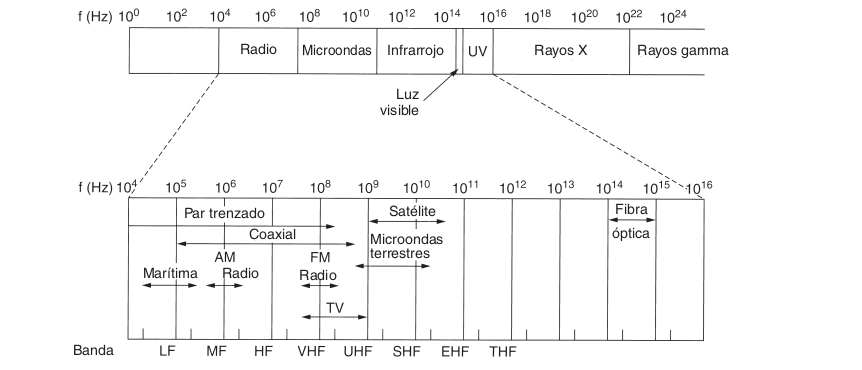
\includegraphics[width=\textwidth
]{images/espectro-magnetico.png}
	\caption[Espector magnetico]{Espector magnetico}
	\label{fig:espectro-magnetico}
\end{figure}

Las porciones de radio, microondas, infrarrojo y luz visible del espectro pueden servir para transmitir información modulando la amplitud, frecuencia o fase de las ondas. La luz ultravioleta, los rayos X y los rayos gamma serían todavía mejores, debido a sus frecuencias más altas, pero son difíciles de producir y modular, no se propagan bien entre edificios y son peligrosos para los seres vivos. 

La cantidad de información que puede transportar una onda electromagnética se relaciona con su ancho de banda. Con la tecnología actual, es posible codificar unos cuantos bits por hertz a frecuencias bajas, pero a frecuencias altas el número puede llegar hasta 8 bits, de modo que un cable coaxial con un ancho de banda de 750 MHz puede transportar varios gigabits/seg.

A las bandas más altas se les nombró como bandas VHF (frecuencia muy alta), UHF (frecuencia ultraalta), EHF (frecuencia extremadamente alta) y THF (frecuencia tremendamente alta).

\subsubsection*{Radio}
Las ondas de radio son fáciles de generar, pueden viajar distancias largas y penetrar edificios sin problemas, y por ello su uso está muy generalizado en la comunicación, tanto en interiores como en exteriores. Las ondas de radio también son  omnidireccionales, lo que significa que viajan en todas direcciones a partir de la fuente, por lo que no es necesario que el transmisor y el receptor se encuentren alineados físicamente.

Las propiedades de las ondas de radio dependen de la frecuencia. A bajas frecuencias, esas ondas cruzan bien casi cualquier obstáculo, pero la potencia se reduce de manera drástica a medida que se aleja de la fuente.

En las bandas VLF, LF y MF las ondas de radio siguen la curvatura de la Tierra. Estas ondas se pueden detectar hasta a 1000 km en las frecuencias más bajas, y a menos en frecuencias más altas.

En las bandas HF y VHF, las ondas a nivel del suelo tienden a ser absorbidas por la tierra. Sin
embargo, las ondas que alcanzan la ionosfera, una capa de partículas cargadas que rodea a la Tierra a una altura de 100 a 500 km, se refractan y se envían de regreso a nuestro planeta. En ciertas condiciones atmosféricas, las señales pueden rebotar varias veces. Los operadores de radio aficionados usan estas bandas para conversar a larga distancia.
El ejército se comunica también en las bandas HF y VHF.

\subsubsection*{Láser}
La señalización óptica coherente con láseres es inherentemente unidireccional, de modo que cada edificio necesita su propio láser y su propio fotodetector. Este esquema ofrece un ancho de banda muy alto y un costo muy bajo. También es relativamente fácil de instalar.

Una desventaja es que los rayos láser no pueden penetrar la lluvia ni la niebla densa, pero normalmente funcionan bien en días soleados. Sin embargo, el calor del sol causa corrientes de convección que se elevabn desde el techo de los edificio. Este aire turbulento desviaba el rayo y lo hacía danzar alrededor del detector.

\subsubsection*{Satélites}
Los satélites de comunicaciones tienen algunas propiedades interesantes que los hacen atractivos para muchas aplicaciones. En su forma más simple, un satélite de comunicaciones se puede
considerar como un enorme repetidor de microondas en el cielo. Contiene numerosos transponedores, cada uno de los cuales se encarga de una parte del espectro, amplifica la señal entrante
y a continuación la retransmite en otra frecuencia para evitar interferencia con la señal entrante.
Los haces pueden ser amplios y cubrir una fracción sustancial de la superficie de la Tierra, o estrechos, y abarcar sólo algunos cientos de kilómetros de diámetro. Este modo de operación se
conoce como de tubo doblado.

\subsection{Red télefonica}
La \textbf{Red Telefónica Pública Conmutada} (PSTN), fue diseñadas hace muchos años, con el propósito de transmitir la voz humana en una forma más o menos reconocible.

\begin{figure}[H]
	\centering
	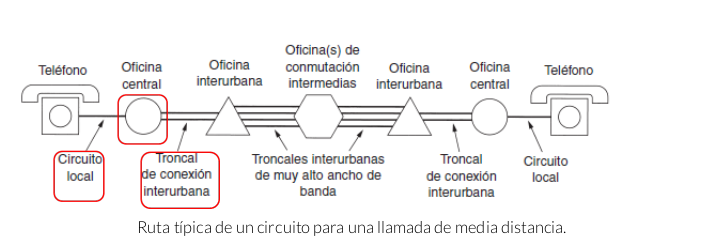
\includegraphics[width=0.9\textwidth
]{images/redes-telefonicas.png}
	\caption[Sistema  telefónico]{Sistema  telefónico}
	\label{fig:sistema-telefonico}
\end{figure}

El sistema telefónico consiste en tres componentes principales:
\begin{enumerate}
  \item Circuitos locales: Cables de par trenzado que van hacia las casas y las empresas. Dan acceso a todo mundo al sistema completo, debido a lo cual son cruciales. Por desgracia, también son la parte más débil del sistema. Cada oficina central tiene varias líneas salientes a uno o más centros de conmutación cercanos, llamados \textbf{oficinas interurbanas}.
  \item Troncales (fibra óptica digital que conecta a las oficinas de conmutación).
  \item Oficinas de conmutación (donde las llamadas pasan de una troncal a otra).
\end{enumerate}

Para las troncales de largo alcance, la principal consideración es cómo reunir múltiples llamadas y
enviarlas juntas por la misma fibra. Este tema se llama \textbf{multiplexión}.

\subsubsection{Tipos de multiplexión}
Las compañías telefónicas han desarrollado esquemas complejos para multiplexar muchas conversaciones en una sola troncal física. Estos esquemas de multiplexión se pueden dividir en dos categorías principales: FDM (Multiplexión por División de Frecuencia) y TDM (Multiplexión por División de Tiempo). En FDM el espectro de frecuencia se divide en bandas de frecuencia, y cada usuario posee exclusivamente alguna banda. En TDM los usuarios esperan su turno (en round-robin), y cada uno obtiene en forma periódica toda la banda durante un breve lapso de tiempo.

\paragraph{Multiplexión por División de Frecuencia:} Los filtros limitan el ancho de banda utilizable a cerca de 3000 Hz por canal de calidad de voz. Cuando se multiplexan muchos canales juntos, se asignan 4000 Hz a cada canal para mantenerlos bien separados. Primero se eleva la frecuencia de los canales de voz, cada uno en una cantidad diferente, después de lo cual se pueden combinar, porque en ese momento no hay dos canales que ocupen la misma porción del espectro. Hay cierta superposición entre canales adyacentes porque los filtros no tienen bordes bien definidos. Esta superposición significa que un pico fuerte en el borde de un canal se detectará en el adyacente como ruido no térmico. Para los canales de fibra óptica se utiliza una variante de la multiplexión por división de frecuencia llamada \textbf{Multiplexión por División de Longitud de Onda} (WDM).

\paragraph{Multiplexión por División de Tiempo:} Aunque FDM aún se utiliza sobre cables de cobre o canales de microondas, requiere circuitos analógicos y no es fácil hacerla con una computadora. En contraste, TDM puede manejarse por completo mediante dispositivos digitales y a ello se debe su popularidad en los últimos años. Desgraciadamente, sólo se puede utilizar para datos digitales. Puesto que los circuitos locales producen señales analógicas, se necesita una conversión de analógico a digital en la oficina central, en donde todos los circuitos locales individuales se juntan para combinarse en troncales.

\subsubsection{Conversión analógico digital}
\begin{figure}[H]
	\centering
	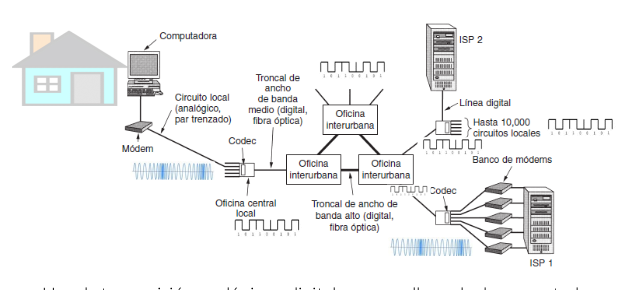
\includegraphics[width=0.9\textwidth
]{images/conversion-analogico-digital.png}
	\caption[Conversión analogico digital]{Conversión analogico digital}
	\label{fig:conversion-analogico-digital}
\end{figure}
\subsection{Modulación}
La transmisión analógica se realiza en una señal continua de frecuencia constante  denomidada \textbf{portadora}. La frecuencia de la portadora se elige de tal forma que sea compatible con las características del medio que se vaya a utilizar. Los datos se pueden transmitir modulando la señal portadora para asegurarnos de que llegue al próximo extremo sin perder información. Todas las técnicas de modulación implican la modificación de uno o más de los tres parámetros fundamentales de la frecuencia portadora: amplitud, frecuencia y fase.

La señal de entrada \(m(t)\) se denomina señal \textbf{moduladora} a la señal resultante de la modulación de la señal portadora.

Hay distintos tipos de modulaciones:

\begin{itemize}
  \item \textbf{Desplazamiento de amplitud (ASK):} Los dos valores binarios se representan mediante dos amplitudes diferentes de la portadora. Es usual que una de las amplitudes sea cero.
  \[
    S(t) = \begin{cases}
      A\cos(2\pi f_c t) & \text{1 binario} \\
      0 & \text{0 binario}
    \end{cases}
  \]

  ASK es sensible a cambios repentinos de la ganancia, además es una técnica de modulación bastante ineficaz. Se usa para la transmición de datos digitales en fibras ópticas.
  \item  \textbf{Desplazamiento de frecuencia (FSK):} Los dos valores binarios se representan mediante dos frecuencias diferentes próximas a la frecuencia portadora. La señal resultante es
  \[
    S(t) = \begin{cases}
      A\cos(2\pi f_1 t) & \text{1 binario} \\
      A\cos(2\pi f_2 t) & \text{0 binario}
    \end{cases}
  \]
  
  donde \(f_1\) y \(f_2\) corresponden a desplazamientos de la frecuencia portadora \(f_c\), de igual magnitud pero en sentidos opuestos.

  FSK es menos sensible a errores que ASK.
  \item  \textbf{Desplazamiento de fase (PSK):} La fase de la señal portadora se desplaza para representar con ello a los datos digitales: En este sistema, un cero binario se representa mediante la transmición de una señal con la misma fase que la fase de la señal anteriormente enviada. Mientras que un uno se representa mediante la transmición de una señal cuya fase esté en opocisión de fase respecto de la señal precedente. Esta técnica se conoce como PSK diferencial, ya que el desplazamiento en fase es relativo a la fase correspondiente al último símbolo transmitido.
  
  \[
    S(t) = \begin{cases}
      A\cos(2\pi f_c t + \pi) & \text{1 binario} \\
      A\cos(2\pi f_c t) & \text{0 binario}
    \end{cases}
  \]
\end{itemize}

\paragraph{Velocidad de modulación:} El número de cambios de señal por unidad de tiempo. Se expresa en \textbf{baudios} (símbolos por segundo).

\paragraph{Velocidad de transmición:} Equivale a la velocidad de modulación multiplicado por el número de bits \(N\) representados por cada símbolo. Se expresa en bits por segundo: \(V_t = V_m\cdot m\)

Se puede conseguir una utilización más eficaz del ancho de banda si cada elemento de señalización representa más de un bit.  En el método PSKQ  se consideran desplazamientos de fase correspondientes a \(\pi/2\) (\(90^\circ\)) por lo que cada señal representa dos bits en lugar de uno:
\[
  S(t) = \begin{cases}
    A\cos(2\pi f_c t + \frac{\pi}{4}) & \text{11} \\
    A\cos(2\pi f_c t + \frac{3\pi}{4}) & \text{10} \\
    A\cos(2\pi f_c t + \frac{5\pi}{4}) & \text{00} \\
    A\cos(2\pi f_c t + \frac{7\pi}{4}) & \text{01} \\
  \end{cases}
\]

\subsubsection{Codificación}
Una vez modulada, la señal analógica viaja hasta un \textbf{codec}  en la oficina central  que se encarga de digitalizarla. El codec toma 8000 muestras por segundo porque el teorema de Nyquist dice que esto es suficiente para capturar toda la información del ancho de banda de 4 kHz del canal telefónico. A una velocidad de muestreo menor, la información se perdería; a una mayor, no se ganaría información extra. Esta técnica se llama \textbf{Modulación por Codificación de Impulsos} (PCM).   

A veces, se usa un técnica conocida como \textbf{Modulación Delta}, en el que la entrada analógica se aproxima mediante una función escalera que en cada intervalo de muestreo (\(T_S\)) sube o baja un nivel de cuantización \(\delta\). La característica principal de la función escalera es que su comportamiento es binario: En cada instante de muestreo, la función sube o baja una cantidad constante. Por tanto, la salida del modulador delta se puede representar mediante un único bit para cada muestra. Resumiendo: se obiente una cadena de bits que aproxima a la derivada de la señal analógica de entrada en cualquier lugar de la amplitud.

\subsubsection*{No retorno a cero (NRZ)}
La forma más frecuente y fácil de transmitir señales digitales es mediante la utilización de un nivel diferente de tensión para cada uno de los dos dígitos binarios. Los códigos que siguen esta estrategia comparten la propiedad de que el nivel de tensión se mantiene constante durante la duración del bit. Es habitual usar un nivel negativo para representar un valor binario y un tensión positiva para representar el otro.

Una variante de este código se nomina \textbf{No retono a Cero con Inversion de unos} (NZRI) en la que un 1 se codifica mediante la transición al principio del intervalo de señalización, mientras que un 0 se representa por la ausencia de transición. Esta codificación es un ejemplo de codificación diferencial, en lugar de determinar el valor absoluto, la señal se codifica comparando la polaridad de los elementos de señal adyacentes.

\subsubsection*{Codificación Manchester (Bifase)}
El valor de un bit se códifica en una transición a la mitad del intervalo de duración del bit. Esta transición en la mitad del bit sirve como un procedimiento de sincronización a la vez que sirve para transmitir los datos: Una transción de bajo a alto representa un 1 y una transición de alto a bajo representa un cero.

En Manchester diferencial, la transición a mitad del intervalo se utiliza tan solo para proporcionar sincronización. La codificación de un cero se representa por la presencia de una trancisión al principio del intervalo. 

Toda técnica bifase fuerza al menos una transición por cada bit pudiendo tener hasta dos en ese mismo período. Por tanto, la velocidad de modulación máxima es el doble que en los NRZ y el ancho de banda necesario es mayor.

\subsection{Redes de conmutación}
En la actualidad se utilizan dos técnicas de conmutación diferentes: conmutación de circuitos y conmutación de paquetes. A continuación presentaremos una breve introducción a cada una de ellas.

\subsubsection*{Conmutación de circuitos}
Cuando se realiza una llamada telefónica, el equipo de conmutación del sistema telefónico busca una trayectoria física que vaya desde su teléfono al del receptor. Esta técnica se llama \textbf{conmutación de circuitos}.

Una propiedad importante de la conmutación de circuitos es la necesidad de establecer una trayectoria de un extremo a otro antes de que se pueda enviar cualquier dato. El tiempo que transcurre entre que se termina de marcar y que el timbre comienza a sonar puede ser fácilmente de 10 seg, y más en las llamadas de larga distancia o internacionales. Durante este intervalo de tiempo, el sistema telefónico busca una trayectoria de cobre. La señal de petición de llamada se debe propagar hasta el destino y se debe confirmar su recepción. En muchas aplicaciones de computadora, los tiempos de establecimiento largos son indeseables.

Por otro lado, al existir una trayectoria de cobre entre las partes en comunicación, una vez que se termina de establecer, el único retardo de los datos es el tiempo de propagación de la señal electromagnética y no
hay peligro de congestión; es decir, una vez que la llamada entra, no hay posibilidad de obtener una señal de ocupado, aunque podría obtener una antes de establecer la conexión debido a la falta de capacidad de conmutación o de troncal.

\subsubsection*{Conmutación de paquetes}
La alternativa a la conmutación de circuitos es la \textbf{conmutación de paquetes}. Con esta tecnología, los paquetes individuales se envían conforme se necesite, y no se les asigna por adelantado ninguna trayectoria dedicada.

En este caso, al no ser necesaria una conexión previa, el primer paquete se puede enviar apenas esté listo. 

Con la conmutación de paquetes no
hay trayectoria, por lo que diferentes paquetes pueden seguir trayectorias distintas, dependiendo
de las condiciones de la red en el momento en el que se enviaron. Pueden llegar en desorden.

La conmutación de paquetes es más tolerante a las fallas que la conmutación de circuitos. De  hecho, ésa es la razón por la cual se inventó. Si falla la conmutación, todos los circuitos que la están utilizando se cancelan y no se puede enviar nada más a través de ellos. Con la conmutación de paquetes, los paquetes pueden enrutarse evitando a los conmutadores averiados.

La conmutación de paquetes utiliza transmisión de almacenamiento y reenvío. Un paquete se
almacena en la memoria del enrutador y luego se reenvía al siguiente enrutador. Con la conmuta-
ción de paquetes los bits simplemente fluyen de manera continua a través del cable. La técnica de
almacenamiento y reenvío agrega retardo.